%%%%%%%%%%%%%%%%%%%%%%%%%%%%%%%%%%%%%%%%%%%%%%%%%%%%%%%%%%%%%%%%%%%%%%%%%%%%
% AGUJournalTemplate.tex: this template file is for articles formatted with LaTeX
%
% This file includes commands and instructions
% given in the order necessary to produce a final output that will
% satisfy AGU requirements, including customized APA reference formatting.
%
% You may copy this file and give it your
% article name, and enter your text.
%
%
% Step 1: Set the \documentclass
%
%

%% To submit your paper:
\documentclass[draft]{agujournal2019}
\usepackage{url} %this package should fix any errors with URLs in refs.
\usepackage{lineno}
\usepackage[inline]{trackchanges} %for better track changes. final new option will compile document with changes incorporated.
\usepackage{soul}
\usepackage{natbib}
\usepackage{amsmath}
\def\permille{\ensuremath{{}^\text{o}\mkern-5mu/\mkern-3mu_\text{oo}}}
\usepackage{lmodern}
\usepackage{float}

% DELETE this part
\usepackage{xargs}
\usepackage[colorinlistoftodos,prependcaption,textsize=tiny]{todonotes}
% 
\newcommandx{\josue}[2][1=]{\todo[linecolor=red,backgroundcolor=red!25,bordercolor=red,#1]{#2}}
\newcommandx{\camille}[2][1=]{\todo[linecolor=blue,backgroundcolor=blue!25,bordercolor=blue,#1]{#2}}
% DELETE up to here

\linenumbers
%%%%%%%
% As of 2018 we recommend use of the TrackChanges package to mark revisions.
% The trackchanges package adds five new LaTeX commands:
%
%  \note[editor]{The note}
%  \annote[editor]{Text to annotate}{The note}
%  \add[editor]{Text to add}
%  \remove[editor]{Text to remove}
%  \change[editor]{Text to remove}{Text to add}
%
% complete documentation is here: http://trackchanges.sourceforge.net/
%%%%%%%

% \draftfalse

%% Enter journal name below.
%% Choose from this list of Journals:
%
% JGR: Atmospheres
% JGR: Biogeosciences
% JGR: Earth Surface
% JGR: Oceans
% JGR: Planets
% JGR: Solid Earth
% JGR: Space Physics
% Global Biogeochemical Cycles
% Geophysical Research Letters
% Paleoceanography and Paleoclimatology
% Radio Science
% Reviews of Geophysics
% Tectonics
% Space Weather
% Water Resources Research
% Geochemistry, Geophysics, Geosystems
% Journal of Advances in Modeling Earth Systems (JAMES)
% Earth's Future
% Earth and Space Science
% Geohealth
%
% ie, \journalname{Water Resources Research}

\journalname{Geophysical Research Letters}

\hfuzz=100pt
\hbadness=10000

\begin{document}

%% ------------------------------------------------------------------------ %%
%  Title
%
% (A title should be specific, informative, and brief. Use
% abbreviations only if they are defined in the abstract. Titles that
% start with general keywords then specific terms are optimized in
% searches)
%
%% ------------------------------------------------------------------------ %%

% Example: \title{This is a test title}

\title{Does the presence of leads in the Arctic sea ice have an impact on the ocean surface?}


%% ------------------------------------------------------------------------ %%
%
%  AUTHORS AND AFFILIATIONS
%
%% ------------------------------------------------------------------------ %%

\authors{Josu\'e Mart\'inez-Moreno\affil{1}, Camille Lique\affil{1}, Claude Talandier\affil{1}}


\affiliation{1}{Univ Brest, CNRS, Ifremer, IRD, Laboratoire d'Oc\'eanographie Physique et Spatiale (LOPS), IUEM, F29280, Plouzan\'e, France.}

\correspondingauthor{Josu\'e Mart\'inez-Moreno}{josue.martinez.moreno@ifremer.fr}

\begin{keypoints}
    \item Buoyancy fluxes in Linear Kinematic Features vary seasonally 
    \item Buoyancy fluxes in Linear Kinematic Features can be 20-30\% larger than in the ice-pack in summer.
    \item The presence of Linear Kinematic Features has a small impact in the transform water masses at the ocean surface.
\end{keypoints}

\begin{abstract}
    The Arctic sea-ice, in particular the ice-pack, acts as an insulator between the atmosphere and the ocean below. Leads, common in Arctic sea ice, facilitate exchanges of heat, salt, moisture and gases between the ocean and the atmosphere. Therefore, leads can influence heat exchanges, ice melt or growth, ocean dynamics, and the atmospheric boundary layer. The existing literature suggests that leads play a significant role in the heat budget of the surface of the ocean and likely impact water mass transformation within the Arctic. However, due to the lack of observations and high resolution models capable to resolve leads, an estimate of the impact of leads in the ocean has been elusive.  Here, we explore the magnitude and impact in the ocean surface caused by the leads using SEDNA, a really high-resolution pan-Arctic hindcast (1/60$^\circ$; NEMO + SI3 configuration). Leads account for $20\%$ of the sea-ice cover area, and within them, there is approximately 20\% of the total surface water mass transformation. 
    The buoyancy flux and water mass transformation in leads are similar to those underneath the surrounding floes and the percentage of WMT through leads matches their area covered. 
    Thus, the present estimate indicates that leads have a small contribution to Arctic Ocean dynamics, contrary to previous hypotheses.
\end{abstract}

\section*{Introduction}

The Arctic sea-ice plays a crucial role in regulating Earth's climate by acting as a natural insulator between the atmosphere and the ocean below \citep{Wettlaufer_insulator_1997, Untersteiner_ice_insulator_1961}. This insulating property acts as a thermal barrier, limiting heat loss from the ocean to the atmosphere, minimizing evaporation, and maintaining the stability of the polar environment \citep{Ruffieux_pack_lead_1995}. A ubiquitous feature of Arctic sea ice is the formation and persistence of leads. Leads are regions where the sea ice deformation reaches a local maxima (See methods for the definition of sea ice deformation; \citealt{Hutter_identification_2019}). These features are characterized by sea ice shear and divergence that can result in an opening of the sea ice, and thus allow large flux exchanges between the ocean and the atmosphere \citep{Lupkes_leads_2008}. Leads vary in width from a few meters to kilometers, with length-scale spanning distances of a few kilometers up to hundreds of kilometers, and generally last from a few hours up to a few days \citep{Linow_lkf_2017, Wernecke_Lead_2015, Tschudi_obs_leads_1998}. Leads can be formed through the divergence or/and shear of the sea ice forced by winds and oceanic currents \citep{Rampal_nextsim_2016, Hutchings_model_lkf_2005, Richter_pack_stress_2002}. Winds are thought to be the main forcing of the sea ice deformation and the formation of leads \citep{Linow_lkf_2017, Hutter_scaling_lkf_2018}. Meanwhile, ocean currents have a smaller contribution to the sea ice deformation compared to wind forcing, but the ocean drag at the bottom of the ice acts to balance the wind-induced sea ice velocities, stabilizing the sea ice cover \citep{Weiss_scale_2004}. Additionally, observations show that ocean currents may play a bigger role in dictating the fracturing patterns of sea ice, since regions with strong currents and bathymetric features are collocated with a larger occurrence of leads \citep{Willmes_leads_currents_2023}. \josue{Rephrased, is it clearer?}

Once leads are formed, atmospheric forcing in conjunction with localized upwelling can result in important heat fluxes at the ocean surface ($\sim 400 W/m^2$; \citealp{McPhee_LKF_2005,Marcq_flux_lead_2012,Maykut_heat_1986}), instigating localized melting/freezing of sea ice \citep{Albedyll_thickness_dis_2022}. Additionally, changes in buoyancy forcing due to brine rejection into the mixed layer can induce convection \citep{Smith_convection_1998}, leading to the generation of fronts, mixed layer turbulence, and eddy generation \citep{Reiser_LKF_2020, Smith_generation_2002}. Furthermore, changes in the buoyancy flux could result in the local transformation the surface water masses \citep{Pemberton_WMT_2015, Smith_polynyas_1990, Walin_WMT_1982}. 
Although all the previous studies have shown that instances of leads can locally impact the ocean dynamics, the overall impact of leads to the ocean dynamics across the Arctic basin are yet to be quantified. \josue{I rephrased, this should be clearer now.}

In-situ observations have provided evidence that leads locally impact the ocean structure of the Arctic Ocean. Nevertheless, the lack of observations limits an estimation of their integrated impact on the Arctic Ocean. Here, we present the first estimate of the impact of the leads in the Arctic Ocean, using a really high-resolution pan-Arctic hindcast, SEDNA \citep{SEDNA_2023}. Since the ice cover is dynamically and thermodynamically different in the marginal ice zone (MIZ) and the ice pack, we differentiate between the leads in each region. Hereafter, we refer to leads as the union of the MIZ leads and the ice pack leads or LKFs. The impact of MIZ leads and ice pack LKFs is quantified by using buoyancy fluxes and the water mass transformation framework (See Methods for details of the calculations and numerical model). 

\subsection*{Lead contribution to the ocean buoyancy}

\begin{figure}
    \centering
    
\includegraphics[width=0.9\textwidth]{./figures/Figure_1_SENTINE_SEDNA_LKF_conc_New_Color.pdf}
    \caption{a) Snapshot of the total deformation for the 21st of April 2014. b) Mean lead frequency between 2011 and 2015. c) True color image from Sentinel 3 on the 12th of April 2022 for the magenta area in panel a. d) Snapshot of the ice concentration from SEDNA on the 21st of April 2014. e) Total deformation used to identify leads. f) Mask of identified leads on the 21st of April 2014.}
    \label{fig:fig1}
\end{figure}

Climate models and coupled models with resolutions lower than $4.5km$ are unable to reproduce many aspects of leads due to the lack of resolution to capture their spatial scale \citep{Wang_leads_2016}. SEDNA is capable of overcoming this limitation and capture most of the lead width distribution ($>1km$; \citealt{Wernecke_Lead_2015}), since the model resolution is $\sim 800m$ on average across the Arctic. 
A snapshot of the total deformation is shown in figure \ref{fig:fig1}a. A closer examination, focusing north of Greenland in panels c, d, e, and f of figure \ref{fig:fig1}, reveals similarities between the spatial pattern of typically observed leads on the 12th of April 2022 from a true color satellite image (Fig. \ref{fig:fig1}c) and the ice concentration of SEDNA for the 21st of April 2014. Note that the sea ice concentration in the identified leads shown in figure \ref{fig:fig1}f using the lead identification algorithm proposed by \citet{Hutter_identification_2019} remains higher than 90\% concentration; this is a consequence of the visco-plastic nature of the sea ice model and the daily averaged output that smooths the presence of leads in the fields. 
Despite this, the similarities between the observations and model lead probability allow us for the first time to estimate quantitatively the impact leads have on the Arctic ocean.

The climatology of the lead probability, i.e. the likelihood of a leads occurring for any given day, is shown in figure \ref{fig:fig1}b. The mean probability of leads averaged over the Arctic is $\sim 19\%$ in SEDNA, comparable to observations using RADARSAT Geophysical Processor System and Thermal-Infrared Satellite Imagery \citep{Wernecke_Lead_2015,Willmes_leads_currents_2023}. Although observations use different identification methods compared to the one implemented in SEDNA \citep{Hutter_identification_2019}, there is resemblance between the spatial patterns of SEDNA and observations (Fig. \ref{fig:S_fig1}). For example, we observe increased lead frequency in the shelves, along bathymetric features, and in regions with large kinetic energy (Fig. \ref{fig:S_fig1}). Several hotspots of lead occurrence can be identified in the Chukchi Sea, highlighting the model's ability to reproduce leads dynamics. SEDNA reproduces the patterns observed in the Arctic shelves, the Greenland Sea, Barents Sea, Kara Sea and Laptev Sea, but the prominent signature in the Beaufort Sea in observations is not captured in SEDNA. 

Figure \ref{fig:fig2}a and b show two snapshots of the buoyancy flux. In winter, a negative buoyancy flux results from sea ice refreezing and brine rejection. In summer, a positive buoyancy flux is associated with sea ice melting and freshening of the Arctic surface (Fig. \ref{fig:fig2}b). Inside the ice covered region (magenta contour) in figure \ref{fig:fig2}, the fluxes are spatially homogeneous, except for the marginal ice zone and the leads, where the buoyancy fluxes are larger than those underneath the surrounding floes, in agreement with previous studies. The flux across the Arctic for the leads is $-2.46\times 10^{-8} m^2/s^3$ and $7.20\times 10^{-8} m^2/s^3$ for each date, respectively, compared to the $-2.42\times 10^{-8} m^2/s^3$ and $5.89\times 10^{-8} m^2/s^3$ underneath the surrounding floes. In other words, in winter, the fluxes across the leads and the surrounding floes are comparable. However, in summer, the fluxes in the leads can be up to 20\% larger than those underneath floes.

\begin{figure}
    \centering
    
\includegraphics[width=1\textwidth]{./figures/Figure_2_buoyancy_flux_maps_vertical_V2.pdf}
    \caption{Maps of buoyancy flux and transects for the 1st of January and 25th of June 2014. a) Map of buoyancy flux on the 1st of January 2014. 
    Transect on the 1st of January 2014 of c) downward heat flux, e) freshwater flux, g) ice thickness and i) buoyancy flux. b) Map of buoyancy flux on the 25th of June 2014. Transect on the 25th of June 2014 of d) downward heat flux, f) freshwater flux, h) ice thickness and j) buoyancy flux. Note that the transect location and orientation changes between the winter and summer dates. Magenta contour in panels a and b correspond to the 0\% concentration contour of sea ice. Vertical blue bars shows the mask of leads in the transect.}
    \label{fig:fig2}
\end{figure}

Two transects across the Beaufort Gyre are shown in figure \ref{fig:fig2} for the 1st of January 2014 and 25th of June 2014.
Examining the 1st of January 2014, we observe a small heat flux in the leads (Fig.\ref{fig:fig2} b), which does not impact the heat flux at the ocean-atmosphere interface since the ocean surface is at freezing point. 
In other words, the extra heat exchanged with the atmosphere is used to form sea ice instead of further cooling the ocean, resulting in a heat flux close to zero at the ocean-ice-atmosphere interface.
In contrast, the salt flux (Fig.\ref{fig:fig2}e) shows two positive peaks, each with twice the magnitude of the surrounding floes, collocated within the identified leads. This is due to an enhanced sea ice growth and brine rejection within the leads. 
The salt flux and heat flux result in a negative buoyancy flux for this snapshot where the largest buoyancy loss occurs within the leads (Fig.\ref{fig:fig2} j). Additionally, within the leads there is a decrease in sea ice thickness of $25cm$ (Fig.\ref{fig:fig2} g). 
On the 25th of June (Fig.\ref{fig:fig2}d), we observe an increase in the heat fluxes within some of the identified leads, reaching up to $\sim 25 W/m^2$. Meanwhile, the freshwater flux shows a local decrease within the leads, indicating a freshening of the surface due to sea ice melt. This change is captured by the positive buoyancy flux, decreasing the density at the surface (Fig.\ref{fig:fig2}k).  The enhanced sea ice melt in the leads results in a sea ice thickness decrease of more than $1m$ within the leads  (Fig.\ref{fig:fig2} h). Note that some peaks in the buoyancy flux align with the edge of the detected leads, likely due to the enhanced refreezing or melting that occur at the edge of the lead. 
Of all the identified leads, some exhibit significant ocean-atmosphere fluxes, while others have little to no imprint in the fluxes. Leads without large ocean-atmosphere fluxes may be explained by the temporality of the sea ice break up (divergence), where later snapshots show an increase of fluxes at the location of identified leads. Alternatively, lead generated through shear and convergence have a limited flux exchange with the atmosphere, but may have enhanced fluxes in the ocean interior due to isopycnal upwelling forced by the ice-ocean stress \citep{Bourgault_flux_lkf_2020}.

Similar to observations, we identify fluxes that are larger in the leads than in the ice pack floes in both summer and winter. However, the freshwater flux, attributable to melting and freezing, is significantly larger than the heat fluxes associated with the leads. In the next section, we explore the impact that leads have in the magnitude of the buoyancy fluxes and water mass transformation across the Arctic basin during 2014. This analysis is conducted separately for the marginal ice zone (MIZ; 0-80\% sea ice concentration), ice pack (80-100\% sea ice concentration) and the leads within each of these regions. 


\subsection*{Mean contribution of leads in the Arctic}

In the Arctic ice covered ocean, the averaged percentage area covered by the four distinct masks representative of the sea ice covered Arctic Ocean during 2014 is as follows: 19\% for the MIZ, 81\% for the ice pack, 14\% for the LKFs in the ice pack, and 10\% for the leads in the MIZ. 
The area covered by each mask exhibit a seasonal cycle (Fig. \ref{fig:fig3}a). During summer (June, July, and August), the percentage of the ice pack cover area decreases from approximately $90\%$ to $50\%$, while the MIZ increases from $10\%$ to approximately $50\%$. 
On one hand, the percentage of the area covered by LKFs in the ice pack peaks in winter (December, January, and February) at almost 20\% coverage over the ice pack area. On the other hand, the leads in the MIZ peak in summer, covering up to 25\% of the total ice cover Arctic and 50\% of the MIZ surface area. The maxima leads area coverage is $\sim 20\%$ of the total sea ice covered Arctic, consistent with previous model assessments \citep{Wang_leads_2016}. 

To quantify the contributions of leads to ocean buoyancy, we integrate the buoyancy flux over each of the sea ice cover masks (Fig. \ref{fig:fig3}b), where the extent of each ice cover mask evolves temporally following the seasonal cycle of the sea ice extent. The buoyancy flux shows a significant seasonal cycle, with positive values corresponding to the sea ice melting season and negative values coinciding with the sea ice freezing season.  
The mean buoyancy flux of the ice pack in winter (December-February) and summer (June-August) is -0.32$m^2/s^3$  and 0.34$\times10^{-14} m^2/s^3$, respectively. The buoyancy flux in the ice pack indicates a shift from ice formation in winter to ice melting in summer, dominated by the haline buoyancy component. Meanwhile, the mean buoyancy flux in the MIZ in winter and summer is 0.01$m^2/s^3$ and 0.25$m^2/s^3$, respectively. A positive buoyancy flux suggests preferential melting across the year in the MIZ, where both thermal and haline component of the buoyancy flux play a role in the MIZ. In both regions, the buoyancy flux in the leads follow the overall seasonal cycle of the buoyancy fluxes underneath the sea ice floes. The buoyancy flux of leads in the MIZ explain 0.003$m^2/s^3$ and 0.13$m^2/s^3$ in winter and summer, respectively. Meanwhile, the buoyancy flux of leads in the ice pack explain -0.05$m^2/s^3$, and 0.07$m^2/s^3$ in winter and summer, respectively. In other words, leads explain between 20-50\% of the buoyancy fluxes in the MIZ and  and between 15-20\% of the buoyancy fluxes in ice pack over the year.
Moreover, the area weighted buoyancy fluxes in figure \ref{fig:fig3}c show that winter leads in the MIZ and the summer leads in the ice pack exhibit larger buoyancy fluxes per unit of area compared to those in the MIZ and ice pack, respectively. 
The mean winter buoyancy flux of the leads in the MIZ is 
-1.98 $\times10^{-14} m^2/s^3$, representing a 40\% larger buoyancy flux in winter within the leads compared to those in the (-1.20 $\times10^{-14} m^2/s^3$), suggesting more freezing within the leads compared to underneath the floes. 
The mean summer buoyancy flux of leads in the ice pack is 7.26$\times10^{-14} m^2/s^3$, approximately 20\% more buoyancy flux in summer compared to the ice pack (5.92$\times10^{-14} m^2/s^3$), indicating enhanced melting with in the ice pack leads. 

\begin{figure}[h!]
    \centering
    
\includegraphics[width=0.9\textwidth]{./figures/Figure_3_buoyancy_flux_components_ts.pdf}
    \caption{Time-series during 2014 of a) the area cover, b) area-weighted  buoyancy fluxes,  c) area-weighted  haline buoyancy flux component, and d) area-weighted thermal buoyancy flux component  for linear kinematic features in the ice pack, the linear kinematic features in the marginal ice zone, the marginal ice zone (ice concentration 0-80\%), and the ice pack (ice concentration $>80\%$).}
    \label{fig:fig3}
\end{figure}

To further quantify the role and impact of leads in the Arctic circulation, we use the surface water mass transformation framework (WMT; \citealp{Walin_WMT_1982}). This approach provides information on the transport of water through the surface density contours due to surface buoyancy forcing that results in the  formation of lighter or denser water at the surface.
In figure \ref{fig:fig4}a, the averaged WMT during 2014 is shown for the ice covered Arctic, the ice pack, the MIZ, and the leads for each of these areas.
The yearly mean WMT in the ice pack is characterized by a broad region of strong positive transformation (losing buoyancy) in halocline polar surface water ($PSW_{H}$; $24.36 kg/m^3 < \rho < 27.41 kg/m^3$), reaching a maximum of $\sim 2.1$ Sv. Additionally, there is a small negative transformation (gaining buoyancy) below $\rho < 23$. 
The yearly mean WMT in the ice pack leads also features a positive peak within the $PSW_{H}$ reaching up to 0.39 Sv. On average the WMT in the ice pack leads accounts for $\sim 10\%$ of the WMT of the ice pack. The MIZ mean WMT is mostly negative within the density range of $20 < \rho < 27.5$ (gaining buoyancy), reaching a minimum of -1.2 Sv around $\rho = 27$.  The MIZ leads WMT is also negative within the same range of densities, with a minimum of -0.6 Sv. On average, the WMT in the MIZ leads corresponds to $\sim 50\%$ of the WMT of the MIZ. Additionally, the sum of the WMT of the ice pack and the WMT of the MIZ, is in agreement with the surface Arctic WMT reported by \citet{Pemberton_WMT_2015}. The transformation of $PSW_{H}$ occurs primarily within the Eurasian basin and a smaller contribution in the Chukchi sea. The transformation of $PSW_{ML}$ ($\rho < 24.36 kg/m^3$) occurs in the Canadian basin, and the $PDW$ and $AW$ ($27.41 kg/m^3 < \rho < 27.81 kg/m^3$ and $27.81 kg/m^3 < \rho$, respectively) occurs in the Barents and Kara seas (Fig.S\ref{fig:S_fig3}). 

Hovmoller diagrams of the seasonal cycle of the WMT during 2014 for the ice pack, the MIZ, and leads in each of these regions are depicted in figure \ref{fig:fig4}.
Overall, in the ice pack and MIZ, winter months show a positive transformation (loss of buoyancy), due to brine rejection during sea ice growth. Meanwhile, summer presents negative transformation or a gain of buoyancy occurs due to the melting of sea ice.  
The mean WMT underneath floes in the ice pack varies from 1.32 Sv in winter and -2.38 Sv in summer, and the WMT in the leads of the ice pack is 0.21 Sv in winter and -0.85 Sv in summer. In other words, the WMT in the ice pack leads explain between 15 to 35\% of the WMT over the year. Furthermore, it is important to note that there is not a emergence of a pattern in the WMT ratios suggesting that LKFs transform the same water masses than those transformed underneath the ice pack floes (\ref{fig:fig4} g). The WMT in MIZ leads in summer is comparable to the summer MIZ WMT.  In winter MIZ leads transform -0.58 Sv, approximately 50\% of the winter MIZ WMT (-1.1 Sv). Similarly to the leads in the ice pack, there is no emergence of a pattern in WMT rations, thus suggesting that the MIZ leads WMT is comparable to the MIZ WMT. 
Overall, the ice covered Arctic, the sum of the ice pack and the MIZ has a mean positive WMT during winter of 1.37 Sv and mean negative WMT of -2.38 Sv during summer (\ref{fig:fig4} b). 
The ice covered lead WMT is 0.27 Sv in winter and -0.85 Sv in summer (\ref{fig:fig4} c). Thus, leads in the ice covered Arctic contribute between 20-35\% of the WMT throughout the year, that corresponds to the area covered by the leads in the ice covered Arctic. 

\begin{figure}[h!]
    \centering
    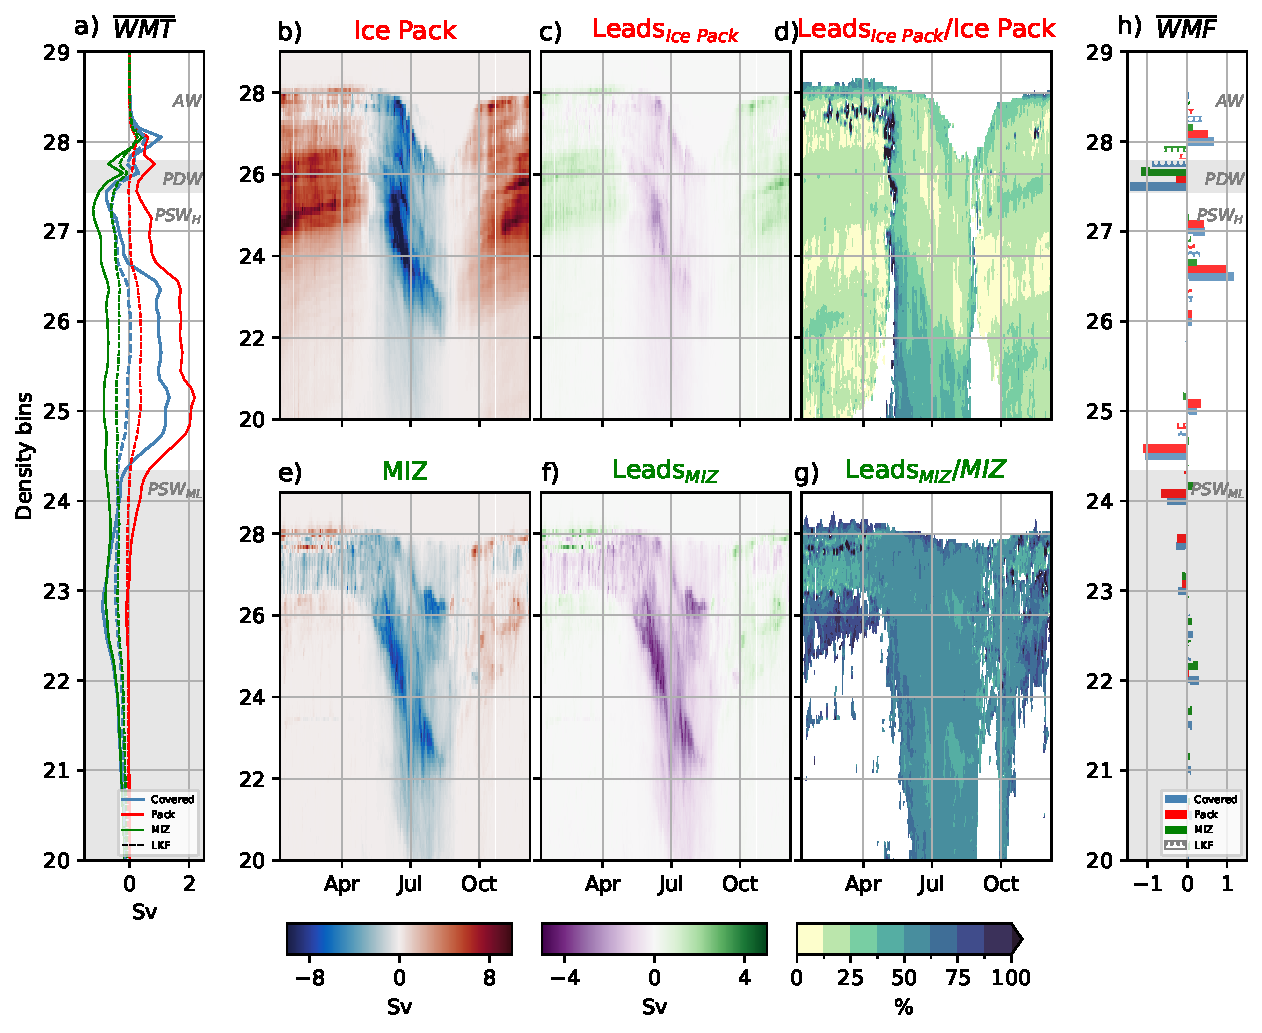
\includegraphics[width=1\textwidth]{./figures/Figure_4_water_mass_transformation_hovmoller_formation_V2.pdf}
    \caption{Mean and daily Water mass transformation over 2014. a) Mean water mass transformation over 2014 for the ice pack, MIZ, and leads in each region. Hovmoller diagram of the water mass transformation (Sv) for the b) ice pack, c) ice pack linear kinematic features and d) the ratio of water mass transformation between the leads and the ice pack region.
    Panels e), f), and g) follow the same structure as panels b), c) and d), but for the MIZ, MIZ leads, and ratio between them.
    h) Mean water mass formation in density bins of $0.5kg/m^3$ during 2014 for the same regions as in panel a). Shaded gray and white areas in panels a) and h) represent the water masses of the Arctic ocean \citep{Pemberton_WMT_2015}: the mixed layer polar surface water ($PSW_{ML}$; $\rho < 24.36 kg/m^3$), the halocline polar surface water ($PSW_{H}$; $24.36 kg/m^3 < \rho < 27.41 kg/m^3$), the polar deep water ($PDW$; $27.41 kg/m^3 < \rho < 27.81 kg/m^3$), and the Atlantic water ($AW$; $27.81 kg/m^3 < \rho$).}
    \label{fig:fig4}
\end{figure}

In figure \ref{fig:fig4}k, the formation rate integrated in $0.5 kg/m^{3}$ density bins for the different ice covered masks, and the leads within each area. The formation rate is the derivative of the mean WMT with respect to the density and it corresponds to the convergence of volume in density space. A negative formation in the upper ocean over a density range indicates that water must be upwelled from the ocean interior or destructed into a different water mass.  We note that there is an agreement in the sign of the water mass formation for each region, this is consistent with the formation of similar water masses in leads and underneath floes. There is a notable destruction of water in the PDW ($27.41 kg/m^3 < \rho < 27.81 kg/m^3$) dominated by the water mass formation in the MIZ and the MIZ leads. This is likely a consequence of ice freezing and melting making a dominant contribution to the destruction in the regions where the PDW outcrops within the MIZ. In contrast, AW ($27.81 kg/m^3 < \rho $) and part of the $\text{PSW}_H$ ($26 kg/m^3 < \rho < 27.41 kg/m^3$) formation occurs principally in the ice pack, with little contribution from the leads. 
Finally, the formation/destruction of other water masses (e.g., $PSW_{ML}$ and lower branch of $\text{PSW}_H$) occur predominantly underneath floes. \josue{I decided to keep this paragraph, since it further helps to say that the formation of water in this regions is not different to those underneath the ice floes.}

\section{Conclusions}

Linear kinematic features are ubiquitous in the sea ice covered oceans that allow exchanges between the ocean and the atmosphere. Generally, the importance of these fluxes at the ocean-atmosphere interface are considered to be of significant importance for the Arctic dynamics \citep{Maykut_solar_1995}. The present study assesses the impact of leads in the ocean surface by diagnosing the buoyancy fluxes using high-resolution hindcast (SEDNA). The lead identification algorithm implemented in SEDNA allows us to reproduce the leads spatial distribution over most regions of the Arctic, with exception of the Beaufort Sea. Despite these regional differences, SEDNA can estimate the mean lead probability, showcasing its capacity to capture the dynamics of these features. This high resolution simulation allows us to better understand the role of leads in shaping the Arctic ocean.

Using SEDNA, we found that leads cover $\sim 20\%$ of the sea-ice covered Arctic, and in the ice pack, leads can contribute up to 20\% more buoyancy flux compared to the fluxes underneath floes. Despite these larger buoyancy fluxes, leads only account for approximately $\sim 20\%$ of the total surface water mass transformation in the ice covered Arctic. Thus, contrary to previous hypotheses, our findings suggest that leads have a small contribution to the transformation of surface water masses and the Arctic Ocean dynamics than previously thought (e.g. \citealp{Hutter_identification_2019, McPhee_LKF_2005}). While their presence can induce localized changes in the density of surface waters due to brine rejection and ice melting, their spatial extent and duration are not sufficient to significantly alter the water masses and link the surface with the ocean interior. Furthermore, both the transformation and formation of water masses in the leads have the same sign, and they are comparable to those underneath the surrounding ice floes. Thus, there is no evidence that leads act differently or that they have a particular imprint in the Arctic ocean water masses.

% \textbf{i not fully sure. As it is, the paragraph does not add much, specially if we do not show the figure in the main part. Maybe that can be a lines or two in the conclusion, to say that additionnaly we axpect change of ekman pumping, surface stress, and primarily MLD within the LKF.. and say we have roughly a 20\% difference?}

A discussed by \citealt{McPhee_LKF_2005}, leads generated by shear can significantly influence in the ocean MLD, by upwelling the isopycnals. Although the MLD is shallower in the leads than underneath the flows in SEDNA (Fig. S\ref{fig:S_fig2}). For example, the difference in MLD between the ice pack and ice pack leads is significant and, on average, the MLD is $\sim 20\%$ shallower during winter in the ice pack leads. This results provides evidence that ice pack LKFs can impact MLD thickness through upwelling, consistent with the observations. This lifting of the MLD in the ice pack leads is likely linked to the ice-ocean stress in LKFs generated by shear, as previously discussed by \citealt{McPhee_LKF_2005, Wettlaufer_insulator_1997, Smith_polynyas_1990}. Nevertheless, there is no evidence of an impact in the ice cover nor a distinct response to the surface buoyancy fluxes or change of the water mass transformation within the leads. Thus, it remains to be investigated if the impact of entrainment in the MLD within the leads, as well as the source of potential energy and generation of instabilities due to isopycnal tilting in the vicinity of leads could impact the Arctic ocean dynamics.

Leads have an important local effect in the atmosphere and the sea-ice fluxes \citep{Lupkes_leads_2008,Marcq_flux_lead_2012}, but a limited imprint in the ocean fluxes. Our results suggest that the representation of leads in oceanic climate models is not prioritary, since there is no evidence in our high-resolution simulation that the fluxes through leads will impact significantly the stratification or the dynamics of the Arctic ocean.
Furthermore, leads are likely to have a negligible implact improving the well known issue within the Arctic climate modeling community of the misrepresentation of the stratification and water masses in the Arctic ocean \citep{Wang_ompi_2024,Ilicak_core_2016}. Finally, a limitation of this study is use of a visco-plastic rheology that results in leads with high ice thickness and  concentrations, thus limiting the exchanges between the ocean and the atmosphere, as compare to the elasto-brittle rheology that may allow larger fluxes through the leads \citep{Rampal_nextsim_2016,Olason_lead_2021}. 


% through the heterogeneous imprint of atmosphere vs sea ice stresses, that likely enhance the fluxes within the leads. Despite this local impact, there is no dominant effect of leads across the Arctic. 


% It has been argued the need of higher resolution tby Current generations of climate models 

% \textbf{Comment in conclusions that the peak in the LKFs is not centered. Only discuss the implication in methods or conclusions.}

% - i think you want to discuss that LKF  may be important dynamically (eg impring the stress)? But it is not clear if the ocean react differently when you have an heterogeneous stress

% - you may want to comment on the implication for climate models. If LKF is 10\% of the WMT, maybe not reasoving them is not the main problem explaining the super bad representation of the stratif/water mass in the Arctic (see the CORE2 papers by wang or Illicak, or the CMIP6 arctic papers


\section{Methods}
\subsection*{Model description}

Here we employ the NEMO numerical platform (release 4.0.5) to establish a 1/60$^\circ$ pan-Arctic ocean-sea ice configuration named SEDNA. The ocean core (NEMO-OCE) solves the primitive equations (PE) using finite differences on an Arakawa C-grid mesh, while the ocean is coupled to the SI3 sea-ice component (NEMO-SI3). The pan-Arctic domain covers the Bering Strait on the Pacific side and extends southward to 56$^\circ$N in the Subpolar North Atlantic gyre and to the Baltic Sea entrance. The ocean model incorporates a linear free surface, utilizes a 3rd order flux form scheme for momentum advection, and employs a 4th order Flux Corrected Transport (FCT) for tracer advection. Additionally, the sea-ice representation includes a 5-category model with the Elasto-Visco-Plastic (EVP) rheology activated and a land-fast capability to better simulate sea-ice behavior in specific areas.

The NCAR bulk formula from Large \& Yeager (2009) to calculate air-sea fluxes and uses hourly ERA5 atmospheric data for near-surface variables. The three lateral boundaries are constrained with daily GLORYS12V1 Re-analysis data, and monthly freshwater fluxes from river discharges are combined with Greenland land ice melt data to supply SEDNA. The simulation extends over seven years (2009 to 2015) and starts from rest, utilizing initial conditions based on the World Ocean Atlas 2009 temperature/salinity and mean January 2009 ice state from PIOMAS re-analysis. Preliminary assessment against available observations and re-analyses data shows that the simulation reasonably captures key ocean and sea-ice characteristics.


\subsection*{Identification of leads}

The leads from SEDNA were identified by using the algorithm proposed by \citet{Hutter_identification_2019}. This method uses the total deformation rate defined as: 
\begin{equation}
    T_d = \left[\left(\underbrace{\frac{\partial u}{\partial x} +\frac{\partial v}{\partial y}}_{Divergence}\right)^2 + \underbrace{\left(\frac{\partial u}{\partial x} - \frac{\partial v}{\partial y}\right)^2+ \left(\frac{\partial u}{\partial y} + \frac{\partial v}{\partial x}\right)^2}_{Shear}\right]^{1/2},
\end{equation}
where $u$ and $v$ are the sea ice velocities. The deformation rate varies spatially depending on the background deformation and the sea ice properties \citep{Reiser_LKF_2020}, where the largest deformation rates occur along the boundaries of ice flows where the leads are found. Therefore, to identify the leads, the local maxima is identified using a DoG filter in the deformation rate field. After this, a binary map is created with the mask of identified lead. Note that after this step, \citet{Hutter_identification_2019} reduce the leads width to a line to then track the leads over time. Since our study focus on the ocean-atmosphere interactions, we only use the identification algorithm to produce a mask of leads during 2014 for the Arctic, where we retain the original width computed from the deformation rate. Finally, the lead mask is then used to quantify and contrast the impact of leads compared to the ice covered Arctic, the ice-pack (ice concentration $> 80\%$) and the MIZ (0 - 80\% ice concentration).

\subsection*{Buoyancy flux and water mass transformation}
 
The Arctic ocean surface experiences large heat and freshwater fluxes, because during the formation of sea ice, salt is rejected and the surface cooled, and when ice melts, freshwater is returned to the ocean and the surface warmed. 
These processes change significantly the surface buoyancy making the surface denser when salt is rejected and lighter when freshwater is added at the surface. This seasonal melt-freeze cycle changes buoyancy and transforms the density of the surface water masses (water mass transformation). \citet{Walin_WMT_1982} proposed the water mass transformation framework that quantifies the rate at which a given water mass is made lighter (negative transformation rate) or denser (positive) due to surface fluxes and mixing. 

The surface water mass transformation is computed as:

\begin{equation}
    \Omega(\sigma_k,t) = \underbrace{- \frac{1}{\sigma_{k+1}-\sigma_k}\iint_A\left(\frac{\alpha Q_{net}}{\rho_0 C_p}\right)dA}_{Net\ surface\ heat\ flux} + \underbrace{\frac{1}{\sigma_{k+1}-\sigma_k}\iint_A\left(\frac{\beta F_{net} SSS }{\rho_0}\right)dA}_{Net\ surface\ freshwater\ flux}
\end{equation}

where $\sigma$ is potential density, $t$ is time, $Q_{net}$ is the net heat flux at the ocean surface, $C_p$ is the specific heat capacity of sea-water, $\beta$ is the haline contraction, $F_{net}$ is the net freshwater flux at the ocean surface and $SSS$ the sea surface salinity. The transformation rate $\omega$ was spatially decomposed into different sea-ice dynamics such as the ice covered, the pack ice, the MIZ, and the leads in each of these regions. 
By separately diagnosing the density transformation that occurs in the leads and underneath the surrounding floes, we quantify the relative importance of the leads for each of these regions. Additionally, this framework accounts for the area changes of the ice cover during the seasonal cycle, and excludes open ocean regions.


\section{Open Research}

\acknowledgments


\bibliography{biblio}

%%% Delete me %%%
\pagebreak
\section*{Appendix}

\renewcommand{\thefigure}{S\arabic{figure}}
\setcounter{figure}{0}
%%% Delete me %%%

\begin{figure}[h]
    \centering
    
\includegraphics[width=1\textwidth]{./figures/comparison_LKF_observations_KE.pdf}
    \caption{Linear kinematic mean frequency from a) Thermal-Infrared Satellite Imagery \citep{Willmes_leads_currents_2023} and b) SEDNA between 2011 and 2015. Panel c) shows the mean kinetic energy between 2011 and 2015.}
    \label{fig:S_fig1}
\end{figure}

\begin{figure}[h]
    \centering
    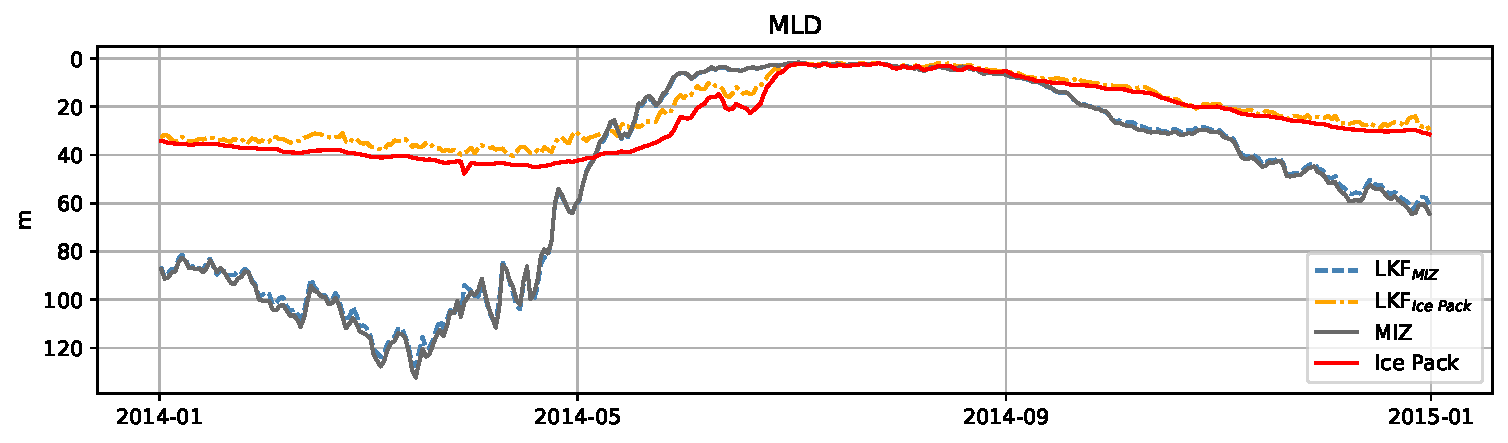
\includegraphics[width=1\textwidth]{./figures/Figure_S2_TS_MLD.pdf}
    \caption{Time-series during 2014 of the mean mixed layer depth for linear kinematic features in the ice pack, the linear kinematic features in the marginal ice zone, the marginal ice zone (ice concentration 0-80\%), and the ice pack (ice concentration $>80\%$). The mixed layer depth is referenced to the first ocean model level.}
    \label{fig:S_fig2}
\end{figure}

\begin{figure}[h]
    \centering
    
\includegraphics[width=1\textwidth]{./figures/Figure_S1_density_maps_season.pdf}
    \caption{Maps of the seasonal surface density of SEDNA during 2014. Magenta contour in maps correspond to the 0\% concentration contour of sea ice.}
    \label{fig:S_fig3}
\end{figure}

\end{document}